\documentclass[11pt, a4paper]{article}

\usepackage{tikz}
\usepackage{amsmath}
\usepackage{amsfonts}
\usepackage{mathtools}
\usepackage{graphicx}
\usepackage{multicol}
\usepackage{appendix}
\usepackage{algorithm}
\usepackage{algpseudocode}
\usepackage[utf8]{inputenc}
\usepackage[english]{babel}

\date{}
\title{Exoplanets detection using \\ auto-tuned random forest}
\author{Lorenzo Loconte}

\begin{document}

\maketitle
\begin{abstract}
  This work consists of identifying exoplanets using random forest which hyperparameters are automatically optimized with techniques that come from the \texttt{AutoML} research.
  The model is trained using the processed data that comes from the \texttt{NASA Kepler} project of discovering exoplanets (i.e. planets outside our solar system).
  The hyperparameters of the model are optimized and cross-validated with \texttt{Hyperband}, a simple yet effective and scalable method for hyperparameters optimization.
  The dataset used in this work can be found at \textbf{https://exoplanetarchive.ipac.caltech.edu}.
\end{abstract}

\section{Introduction}
  \paragraph{Kepler Object of Interest}
    The dataset used in this work is the cumulative list of the \texttt{Kepler Object of Interest} (\texttt{KOI}) tables that come from the \texttt{NASA Kepler} project of discovering exoplanets.
    The dataset is composed by a list of examples regarding exoplanets. Each example have a label indicating if the corresponding exoplanet is candidate, false positive or confirmed. The provided dataset consists of a lot of heterogeneous features. For the classification task the selected features can be found in Appendix \ref{appendix:features}. The candidate exoplanets (i.e. the exoplanets which existence is uncertain) are discarded in order to reduce noise and improve the learning process.
    For simplicity all the examples having null values are removed from the dataset. Furthermore, all the selected features are numeric and the preprocessing method applied to the dataset is the standard normalization.
    The resulting dataset contains \texttt{6884} samples, which \textasciitilde \texttt{67\%} are false positives and the remaining are confirmed.
    
  \paragraph{Random Forests}
    The model used for the classification task is a random forest, a bagging ensemble of decision trees. The prediction of the random forest is computed as the mode of the predictions made by the decision trees. Each tree of the forest is trained on a subset of the features. Random forests correct the habit of decision trees of overfitting on their training set. In fact decision trees tend to overfit their training sets because they have a low bias but an high variance. So, random forests generally obtain a better performance because they reduce the variance, with a little increase of bias due to the \texttt{Bias-Variance} tradeoff. The hyperparameters of the random forest are optimized and cross-validated using approaches that come from the \texttt{AutoML} research. The following hyperparameters are optimized:
    \begin{itemize}
      \item The split criterion (Gini impurity or information gain, see Appendix \ref{appendix:splitcriterions} for details)
      \item The fraction of features to use for each tree
      \item The maximum depth of each tree
      \item The minimum number of samples required to split an internal node
      \item The minimum number of samples to be at a leaf node
    \end{itemize}
  As the next section will expose, the number of trees in the random forest is not considered an hyperparameter because it represents the budget of the hyperparameters optimization algorithm chosen. In this work we refer with budget as the computational cost of cross-validating a certain model.

\section{Hyperparameters Tuning}
  In this section it will be shown a formalization of the hyperparameters optimization task as a search problem. In this work we refer to hyperparameters as the ones that cannot be trained (e.g. the ones described in the previous section). After that we briefly introduce the hyperparameters optimizer used in this work, \texttt{Hyperband}, as described in \cite{hyperband}.

  Given a training set $T$, a model $L$ and its hyperparameters search space $\Omega$, the hyperparameters optimization task consists to find an hyperparameters configuration $\omega \in \Omega$ such that the resulting model $L\langle\omega\rangle$ maximizes a certain score $S$ using cross-validation on $T$.

  There are a lot of different techniques for hyperaparameters optimization, some of them are the following:
  \begin{itemize}
    \item Random Search
    \item Grid Search
    \item Hyperband
    \item Bayesian Optimization
    \item Hybrid Approaches (like \texttt{BOHB} \cite{bohb})
  \end{itemize}

  Of the techniques cited above only \texttt{Bayesian Optimization} guarantees the convergence to the global maximum in the hyperparameters search space (see \cite{bayesianoptimization} for details). The simplest algorithm is \texttt{Random Search} and it works well if the hyperparameters search space is not too big. \texttt{Random Search} is expensive because each evaluation of the score function is done on models completely built from scratch. So, each evaluation of the score function on some randomly selected hyperparameters will use the same amount of computational resources, even if some hyperparameters of the search space obtain a very low score. The idea behind \texttt{Hyperband} is that it's better to save up resources on these hyperparamters configurations that doesn't obtain a sufficiently good score by gradually building more complex models over time.
  
  As we said before we refer to budget as the computational cost of cross-validating a certain model. For example, for neural networks the budget can be the number of training epochs, while for random forests it can be the number of trees.

  \begin{algorithm}
    \caption{Hyperband algorithm for hyperparameters optimization}
    \label{algorithm:hyperband}
    \begin{algorithmic}[1]
      \Procedure{Hyperband}{$T,L,S,\Omega,R,\eta$}
        \State $C \gets \emptyset$
        \State $s_{max} \gets \lfloor \log_{\eta}{R} \rfloor, \quad B \gets (s_{max} + 1)R$
        \For{$s \in \{s_{max},s_{max}-1,...,0\}$}
          \State $n \gets \lceil \frac{B}{R}\frac{\eta^{s}}{(s+1)} \rceil, \quad r \gets R\eta^{-s}$
          \State $H \gets getRandomHyperparameters(n,\Omega)$
          \For{$i \in \{0,...,s\}$}
            \State $n_{i} \gets \lfloor n\eta^{-i} \rfloor, \quad r_{i} \gets r\eta^{i}$
            \State $H \gets top_{\lfloor n_{i}/\eta \rfloor} \arg sort_{\omega} \{S(L\langle\omega \cup \{r_{i}\}\rangle, T) \mid \omega \in H\}$
          \EndFor
          \State $C \gets C \cup H$
        \EndFor
        \State \textbf{return} $\arg max_{\omega} \{S(L\langle\omega \cup \{R\}\rangle, T) \mid \omega \in C\}$
      \EndProcedure
    \end{algorithmic}
  \end{algorithm}

  The algorithm above shows an implementation of \texttt{Hyperband} as desribed now. Given a budget $R$, \texttt{Hyperband} consists of random sampling some points (using an uniform distribution) in the hyperparameters space and cross-validating them using only a fraction of the budget $R$. After that we pick a fraction $1/\eta$ of the best models. In this way we discard the models that didn't obtain a sufficiently good score saving up computational resources. After that we strengthen the previous models using a larger portion of $R$ and iterate in this way until we use the complete budget $R$. The procedure of consequently eliminating hyperparameters samples that don't obtain a good score is called \texttt{Successive Halving}. The fraction of the budget to use for each iteration grows geometrically in respect of $\eta$.

  The remaining problem is to determinate the number of initial random points of the hyperparameters space to sample and the initial budget to use. Generally the number of initial random points is $\eta^{\lfloor \log_{\eta}R \rfloor}$ and the initial budget is set to $R\eta^{-\lfloor \log_{\eta}R \rfloor}$. Furthermore, we execute the discussed algorithm multiple times using less and less initial random points and using an higher starting budget. So, initially \textit{exploration} is preferred and \textit{exploitation} is performed later.

  Even if \texttt{Hyperband} is a simple algorithm, it is well scalable on multiple CPUs because we assume that every point in the hyperparameters space is independent from the others.

  In our case the model $L$ is a random forest. As said before, the budget is the maximum number of trees that the final random forest will have. The choice of the score $S$ is dependent from the target task. For simplicity the $F_{1}$ score is used (i.e. we want to maximize both \textit{Precision} and \textit{Recall}). In this work the hyperparameters search space can be defined formally as:
  \[\Omega = \overbrace{\{gini, entropy\}}^{\text{Split Criterion}} \quad\times \overbrace{(0, 1]}^{\text{Features fraction}} \times\]
  \[\times \overbrace{\mathbb{N}^{*}}^{\text{Max depth}} \times \overbrace{\mathbb{N}^{*}}^{\text{Min samples to split}} \times \overbrace{\mathbb{N}^{*}}^{\text{Min samples at leaf}}\]
  For obvious reasons only a subset of this space can be explored. Table \ref{table:hyperparameters} shows the subset of the hyperparameters search space used in this work.

  The result of the hyperparameters optimization task is a point in the hyperparameters space:
  \[\omega=(c, p, h, k, t)\in\Omega\]
  where $c$ is the split criterion, $p$ is the features fraction for each tree, $h$ is the maximum depth, $k$ is the minimum number of samples to split and $t$ is the minimum number of samples at a leaf, such that the random forest built $L\langle\omega\rangle$ maximize the cross-validation score $S$ on the training set $T$.

  \begin{table}[b]
    \centering
    \begin{tabular}{|c c|}
      \hline
      Hyperparameters & Values \\
      \hline\hline
      Split Criterions & $\{gini, entropy\}$ \\
      \hline
      Features fraction & $(0, 1]$ \\
      \hline
      Maximum Depth & $\{8,9,...,32\}$ \\
      \hline
      Minimum samples to split & $\{2,3,...,16\}$ \\
      \hline
      Minimum samples at a leaf & $\{1,2,...,5\}$ \\
      \hline
    \end{tabular}
    \caption{The hyperparameters space subset used in this work.}
    \label{table:hyperparameters}
  \end{table}

\section{Conclusion}
  As you can see from Table \ref{table:benchmark} the auto-tuned random forest used in this work obtained a way better \textit{Precision} and \textit{Recall}. As you can see from Table \ref{table:confusion} the false positives count (the number of examples, which are predicted as exoplanets, but that are not) and the false negatives count (the number of actual exoplanets not being discovered), are pretty low. At contrary of other models, like neural networks, that are \textit{black-box} models, random forests is a \textit{white-box} model: the predictions can be explained deeply and it is possible to evaluate the importance of each feature used for predictions. In the end we present Table \ref{table:importances} that shows the importances of the first five out fifteen features used.

  \begin{table}
    \centering
    \begin{tabular}{|c c c c|}
      \hline
      Model & Precision & Recall & $F_{1}$  \\
      \hline\hline
      k-NN & 0.700 & 0.832 & 0.757 \\
      \hline
      SVC & 0.775& 0.854 & 0.808 \\
      \hline
      2-layer NN & 0.830 & 0.852 & 0.838 \\
      \hline
      \textbf{Random Forest} \texttt{w/Hyperband} & \textbf{0.866} & \textbf{0.874} & \textbf{0.870} \\
      \hline
    \end{tabular}
    \caption{\textit{Precision}, \textit{Recall} and $F_{1}$ metrics of several models for comparison. The models hyperparameters are the default ones implemented in \texttt{sklearn}. For \texttt{Hyperband} $R=216$ and $\eta=3$ are used.}
    \label{table:benchmark}
  \end{table}
  
  \begin{table}
    \centering
    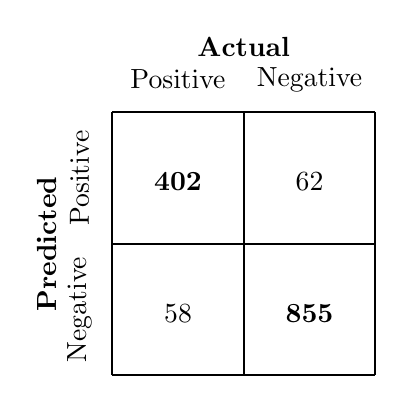
\begin{tikzpicture}[scale=1.67]
      \draw[thick] (0, 0) -- (2, 0);
      \draw[thick] (0, 0) -- (0, 2);
      \draw[thick] (2, 2) -- (2, 0);
      \draw[thick] (2, 2) -- (0, 2);
      \draw[thick] (0, 1) -- (2, 1);
      \draw[thick] (1, 0) -- (1, 2);
      \node[rotate=0] (h1) at (1, 2.5) {\textbf{Actual}};
        \node[rotate=0] (h11) at (0.5, 2.25) {Positive};
        \node[rotate=0] (h12) at (1.5, 2.25) {Negative};
      \node[rotate=90] (h2) at (-0.5, 1) {\textbf{Predicted}};
        \node[rotate=90] (h21) at (-0.25, 1.5) {Positive};
        \node[rotate=90] (h22) at (-0.25, 0.5) {Negative};
      \coordinate[label={\textbf{402}}] (PP) at (0.5, 1.33);
      \coordinate[label={ 58}] (NP) at (0.5, 0.33);
      \coordinate[label={ 62}] (PN) at (1.5, 1.33);
      \coordinate[label={\textbf{855}}] (NN) at (1.5, 0.33);
    \end{tikzpicture}
    \caption{Confusion matrix over the test set.}
    \label{table:confusion}
  \end{table}

  \begin{table}
    \centering
    \begin{tabular}{|c c c|}
    \hline
    Feature \# & Description & Importance \\
    \hline\hline
    5 & Planetary Radius & 0.276 \\
    1 & Orbital Period & 0.162 \\
    4 & Fitted Stellar Density & 0.087 \\
    3 & Transit Depth & 0.085 \\
    6 & Inclination & 0.071 \\
    \hline
    \end{tabular}
    \caption{Features importances in descending order.}
    \label{table:importances}
  \end{table}

\appendix
\appendixpage

\section{Exoplanet Features}
  \label{appendix:features}
  \begin{multicols}{2}
    \begin{enumerate}
      \item Orbital Period [$days$]
      \item Transit Duration [$hrs$]
      \item Transit Depth [$ppm$]
      \item Fitted Stellar Density [$g/cm^{3}$]
      \item Planetary Radius [$Earth\:radii$]
      \item Inclination [$deg$]
      \item Equilibrium Temperature [$K$]
      \item Insolation Flux [$Earth\:flux$]
      \item Stellar Effective Temperature [$K$]
      \item Stellar Surface Gravity [$\log_{10}(cm/s^{2})$]
      \item Stellar Radius [$Solar\:radii$]
      \item Stellar Mass [$Solar\:mass$]
      \item RA [$decimal\:degrees$]
      \item Dec [$decimal\:degrees$]
      \item Kepler-band [$mag$]
    \end{enumerate}
  \end{multicols}

\section{Decision tree split criterions}
  \label{appendix:splitcriterions}
  \subsection{Gini impurity}
    Citing \texttt{wikipedia.org}, Gini impurity is a measure of how often a randomly chosen element from the set would be incorrectly labeled if it was randomly labeled according to the distribution of labels in the subset. To compute Gini impurity for a set of items with $J$ classes, suppose $i\in\{1,2,...,J\}$, and let $p_{i}$ be the faction of items labeled with class $i$ in the set.
    \[{I} _{G}(p)=\sum _{i=1}^{J}p_{i}\sum _{k\neq i}p_{k}=\sum _{i=1}^{J}p_{i}(1-p_{i})=\sum _{i=1}^{J}p_{i}-\sum _{i=1}^{J}{p_{i}}^{2}=1-\sum _{i=1}^{J}{p_{i}}^{2}\]
  \subsection{Information gain}
    Information gain is based on the concept of entropy and information content from information theory. For each node of the tree, the information value represents the expected amount of information that would be needed to specify whether a new instance should be classified yes or no, given the example reached that node. Given $T$ the set of training examples, suppose $i\in\{1,2,...,J\}$, where $J$ is the number of classes, and let $p_{i}$ be the faction of items labeled with class $i$ in the training set.
    \[IG(T, a)=\mathrm{H}(T)-\mathrm{H}(T|a)=-\sum _{i=1}^{J}p_{i}\log _{2}{p_{i}}-\sum _{a}{p(a)\sum _{i=1}^{J}-\Pr(i|a)\log _{2}{\Pr(i|a)}}\]

\bibliography{biblio.bib}
\bibliographystyle{unsrt}

\end{document}
